\section{Алгоритм рендеринга черной дыры}
\label{sec:Chapter1} \index{Chapter1}

Рендеринг реалистичного изображения в компьютерной графике можно сравнивать с фотосъемкой. И там, и там конечным результатом является изображение, которое получается на основании свойств света, попавшего в камеру. Пользуясь этим, можно упростить законы выбранного неевклидова пространства, используя их только для света (фотонов).

Целью данной главы является построение алгоритма рендеринга черной дыры, результатом которого является итоговый цвет.

Многое из описанного в этой главе повторяет уже исследованные методы рендеринга черной дыры: \cite{bruneton2020}, \cite{SHolloway_2020}, \cite{Riazuelo_2019} и других перечисленных в списке литературы. Однако для полноценного понимания настоящей работы алгоритм рендеринга черной дыры будет описан с самого начала.

\subsection{Метрика Шварцшильда}

В науке наиболее популярным методом описания пространства-времени общей теории относительности является метрика - 4-тензор, посредством которого выражается пространственно-временной интервал $ds$. Иначе говоря, благодаря метрике можно понять как при малых изменениях локальных (то есть применимых только в локальной области) координат $(dx, dy, ...)$ изменяется расстояние $ds$ между точками в пространстве. Примеры метрик:
\begin{itemize}
  \item Евклидова: $ds^2=dx^2+dy^2+dz^2$.
  \item Сферическая (двумерная): $ds^2=dx^2+cos^2(\frac{y}{R})dy^2$.
  \item Минковского: $ds^2=c^2dt^2-dx^2-dy^2-dz^2$.
\end{itemize}

Для описания выбранной рабочей сцены, то есть для черной дыры (предполагая, что она не заряжена и не вращается), существует метрика Шварцшильда в сферических координатах $(t, r, \theta, \phi)$:
\begin{equation}
\label{eq:schwarzschild_metric}
    ds^2 = c^2d\tau^2 = \left(1-\frac{r_s}{r}\right)c^{2}dt^{2} - \left(1-\frac{r_s}{r}\right)^{-1}dr^2 - r^2\left(d\theta^2+sin^2(\theta)d\phi^2\right)
\end{equation}
, где $\tau$ - собственное время и $r_s = \frac{2GM}{c^2}$ - \textit{радиус Шварцшильда}, который определяет область вокруг черной дыры массой $M$, которую луч света покинуть не сможет. Считаем, что центр черной дыры расположен в начале координат.

Для частиц в течение движения сохраняются энергия и угловой момент (константы движения):
\begin{equation}
\label{eq:motion_constant_E}
    E = \left(1-\frac{r_s}{r}\right)\frac{dt}{d\tau}.
\end{equation}

\begin{equation}
\label{eq:motion_constant_L}
    L = r^2\frac{d\phi}{d\tau}.
\end{equation}

Метрику можно преобразовать из \eqref{eq:schwarzschild_metric}, считая $c = 1$ и $\theta=\frac{\pi}{2}$, поскольку метрика Шварцшильда симметрична, а значит траектория луча всегда будет лежать в плоскости:
\begin{equation}
\label{eq:schwarzschild_metric1}
    c^2 = \left(1-\frac{r_s}{r}\right)c^2\left(\frac{dt}{d\tau}\right)^2 - \left(1-\frac{r_s}{r}\right)^{-1}\left(\frac{dr}{d\tau}\right)^2 - r^2\left(\frac{d\phi}{d\tau}\right)^2.
\end{equation}

Из \eqref{eq:motion_constant_E}, \eqref{eq:motion_constant_L} и \eqref{eq:schwarzschild_metric1} можно получить следующее выражение:
\begin{equation}
\label{eq:schwarzschild_metric2}
    \left(\frac{dr}{d\tau}\right)^2 = \frac{E^2}{m^2c^2} - \left(1-\frac{r_s}{r}\right)\left(c^2+\frac{L^2}{r^2}\right).
\end{equation}

Поскольку справедливо следующее равенство:
\begin{equation}
\label{eq:equation_of_diff}
    \left(\frac{dr}{d\phi}\right)^2 = \left(\frac{dr}{d\tau}\right)^2\left(\frac{d\tau}{d\phi}\right)^2 = \left(\frac{dr}{d\tau}\right)^2\left(\frac{r^2}{L}\right)^2.
\end{equation}

То используя \eqref{eq:schwarzschild_metric2} и \eqref{eq:equation_of_diff} можно получить уравнение:
\begin{equation}
\label{eq:schwarzschild_metric3}
    \left(\frac{dr}{d\phi}\right)^2 = \frac{r^4}{b^2} - \left(1-\frac{r_s}{r}\right)\left(\frac{r^4}{a^2} + r^2\right).
\end{equation}
, где $a = \frac{L}{c}$ и $b = \frac{mcL}{E}$ - константы.

Применяя замену переменной $u = \frac{1}{r}$, а также учитывая, что при стремлении массы частицы $m$ к нулю, $m \longrightarrow 0$, константа движения $a$ стремиться к бесконечности, $a \longrightarrow \infty$, упрощаем \eqref{eq:schwarzschild_metric3}:
\begin{equation}
\label{eq:schwarzschild_metric4}
    \left(\frac{du}{d\phi}\right)^2 = r_su^3 - u^2 + \frac{1}{b^2}.
\end{equation}

Дифференцируя \eqref{eq:schwarzschild_metric4}:
\begin{equation}
\label{eq:schwarzschild_metric5}
    2\frac{du}{d\phi}\frac{d^2u}{d\phi^2} = 3r_su^2\frac{du}{d\phi} - 2u\frac{du}{d\phi}.
\end{equation}

Итоговый результат из \eqref{eq:schwarzschild_metric5} выглядит следующим образом:
\begin{equation}
\label{eq:diffur}
    \frac{d^2u}{d\phi^2} = \frac{3}{2}r_su^2 - u.
\end{equation}

\subsection{Методы Рунге-Кутты}
\label{subsec:runge-kutte}

Дифференциальное уравнение \eqref{eq:diffur} не имеет явного решения, поэтому разумно использовать для его решения итеративный подход. Таким образом траектория (луч) света будут приближены итеративными точками (см. рис. \ref{fig:runge-kutte}).

\begin{figure}[h]
    \centering
    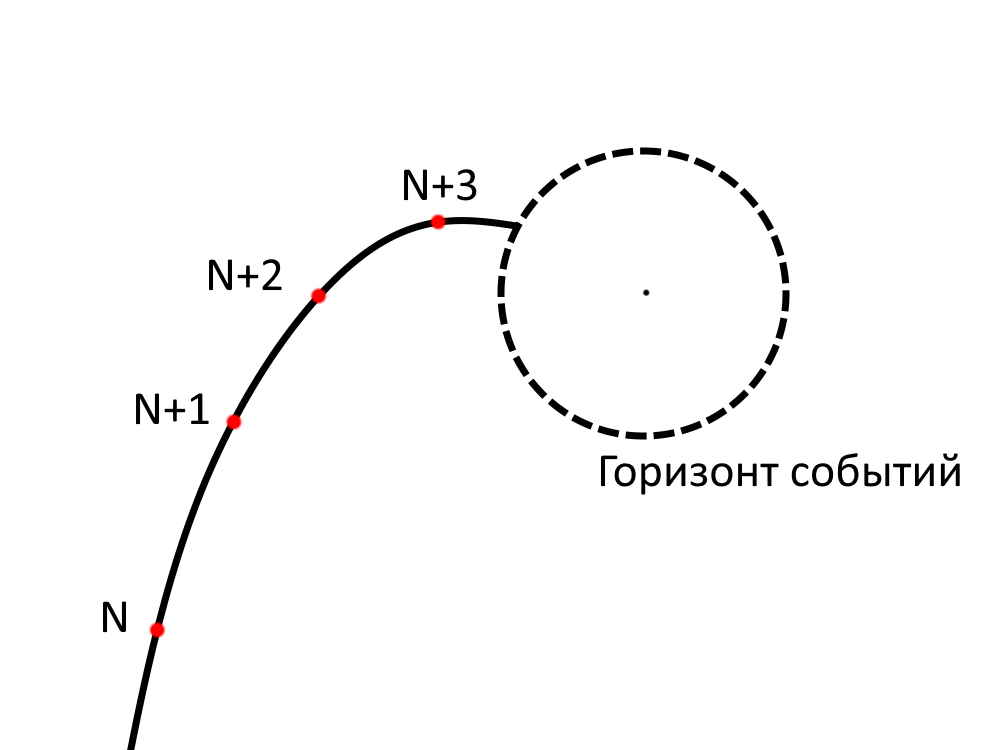
\includegraphics[width=0.8\linewidth]{BlackHole-RayMarching-Overview}
    \caption{Черной сплошной линией показана теоретическая траектория луча света в окрестности черной дыры, а красными точками - итерации метода Рунге-Кутты.}
    \label{fig:runge-kutte}
\end{figure}

Одними из итеративных подходов являются методы Рунге-Кутты \cite[стр.~219]{аристова2014практические}, позволяющие находить решение дифференциальных уравнений с заданными условиями на сетке $\phi$ значений, в общем случае с переменным шагом $\Delta \phi$:

\begin{equation}
\label{eq:runge-kutte}
    \frac{\mathbf{dy}}{d\phi} = \mathbf{f}(\phi, \mathbf{y}),
    \quad
    \left.\mathbf{y}\right|_{\phi=\phi_0}=\mathbf{y_0}.
\end{equation}

В случае уравнения \eqref{eq:diffur}:

\begin{equation*}
\label{eq:runge-kutte_y}
    \mathbf{y} =
    \begin{cases}
        u
        \\
        \frac{du}{d\phi}
    \end{cases}
\end{equation*}

\begin{equation*}
\label{eq:runge-kutte_f}
    \mathbf{f}(\phi, \mathbf{y}), =
    \begin{cases}
        \frac{du}{d\phi}
        \\
        \frac{3}{2}r_su^2 - u
    \end{cases}
\end{equation*}

Для данной работы были выбраны явные методы Рунге-Кутты порядков 1, 2 и 4. Разные порядки имеют разную точность, сведения представлены в таблице \ref{tab:runge-kutte}:

\begin{center}
    \begin{table}[h!]
        \centering
        \begin{tabular}{|c|c|}
            \hline
            Порядок метода Рунге-Кутты & Погрешность шага $\Delta h$ \\
            \hline
            Рунге-Кутты 1-го порядка (RK1) & $O(h^2)$ \\
            \hline
            Рунге-Кутты 2-го порядка (RK2) & $O(h^3)$ \\
            \hline
            Рунге-Кутты 4-го порядка (RK4) & $O(h^5)$ \\
            \hline
        \end{tabular}
        \caption{Сравнение погрешностей методов Рунге-Кутты.}
        \label{tab:runge-kutte}
    \end{table}
\end{center}


\subsection{Инициализация лучей света}
\label{subsec:ray_init}

Для использования методов Рунге-Кутты необходимо определить начальные условия $y_0$ и $\phi_0$ из \eqref{eq:runge-kutte}. Начальное условие $y_0$ будут определяться на основе позиции и направления камеры (то есть наблюдателя), угла обзора (field of view), а также позиции пикселя в изображении.

\begin{figure}[h]
    \centering
    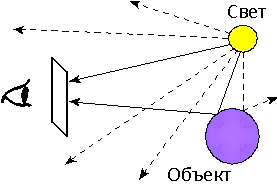
\includegraphics[width=0.5\linewidth]{CameraRaysProblem}
    \caption{Малая часть испущенного света попадает в камеру.}
    \label{fig:camera_rays_problem}
\end{figure}

Стоит отметить, что, как было сказано выше, рендеринг - это свет попавший в камеру. Но испускать свет в сцене от всех источников освещения, а затем учитывать только тот свет, что попал в камеру - невыгодно, поскольку лишь малая часть действительно попадет в камеру (см. рис. \ref{fig:camera_rays_problem}). Поэтому в компьютерной графике давно используют закон обратимости света: гораздо выгоднее выпускать лучи из каждого пикселя камеры и затем просчитывать какой цвет они приобретут в ходе движения по сцене.

\begin{figure}[h]
    \centering
    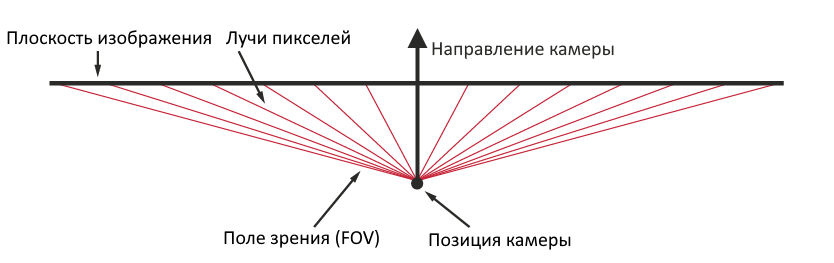
\includegraphics[width=1.0\linewidth]{PinholeCameraModel}
    \caption{Модель камеры-обскуры (pinhole camera model).}
    \label{fig:pinhole_camera}
\end{figure}

В качестве модели камеры выбрана модель камеры-обскуры \linebreak(pinhole camera model) \cite[стр.~47]{marrs2021ray}, поскольку это одна из стандартных моделей камеры. Для ее настройки необходимо знать параметры камеры и угол обзора (поле зрения). Главным следствием использования этой модели является эквидистантность точек пересечения лучей с плоскостью изображения, лежащих на одной линии (см. рис. \ref{fig:pinhole_camera}).

Пусть итоговое изображение, которое будет передано на дисплей, имеет размер $(N, M)$. Индекс пикселя это упорядоченный набор двух неотрицательных чисел $(n, m)$, начиная с $0$ по каждому пикселю. Направление и позиция в декартовых координатах, а также угол обзора камеры обозначаются $\mathbf{d_c}$, $\mathbf{a_c}$ и $fov$ соответственно. В терминологии данной работы углом обзора будет называться угол между крайними лучами на одной горизонтальной прямой. Зная все это можно получить направления лучей каждого пикселя в декартовых координатах $\mathbf{d_0}$:

\begin{align*}
    x &= (n + 0.5)/N, \\
    y &= (m + 0.5)/M, \\
    \text{scale}_{horizontal} = \text{scale}_h &= \tan{\left(\frac{fov}{2}\right)}, \\
    \text{scale}_{vertical} = \text{scale}_v &= \left(\frac{N}{M}\right) \cdot \text{scale}_h, \\
    \mathbf{offset}_{horizontal} = \mathbf{offset}_h &= \text{scale}_h \cdot \left(\frac{\mathbf{d_c} \times \mathbf{e_z}}{\left|\mathbf{d_c} \times \mathbf{e_z}\right|}\right), \\
    \mathbf{offset}_{vertical} = \mathbf{offset}_v &= \text{scale}_v \cdot \left(\frac{\mathbf{d_c} \times \mathbf{offset_h}}{\left|\mathbf{d_c} \times \mathbf{offset_h}\right|}\right).
\end{align*}

Таким образом, направление луча пикселя в декартовых кооринатах $\mathbf{d_0}$ можно вычислить следующим образом:

\begin{equation}
\label{eq:init_rays}
    \mathbf{d_{nm}} = \mathbf{d_c} + \mathbf{offset}_{h} \cdot x + \mathbf{offset}_{v} \cdot y.
\end{equation}

\subsection{Переход из декартовых в полярные координаты плоскости вращения}
\label{subsec:transition_from_decart_to_polar}

Начальные условия $\mathbf{d_0}$ из \eqref{eq:init_rays} получены в декартовых координатах, а метод Рунге-Кутты, изложенный в разделе \ref{subsec:runge-kutte}, описан в полярных координатах. Поэтому перед итеративным решением необходимо определить $y_0$ и $\phi_0$ из \eqref{eq:runge-kutte} на основании данных раздела \ref{subsec:ray_init}.

\newpage

\begin{figure}[h]
    \centering
    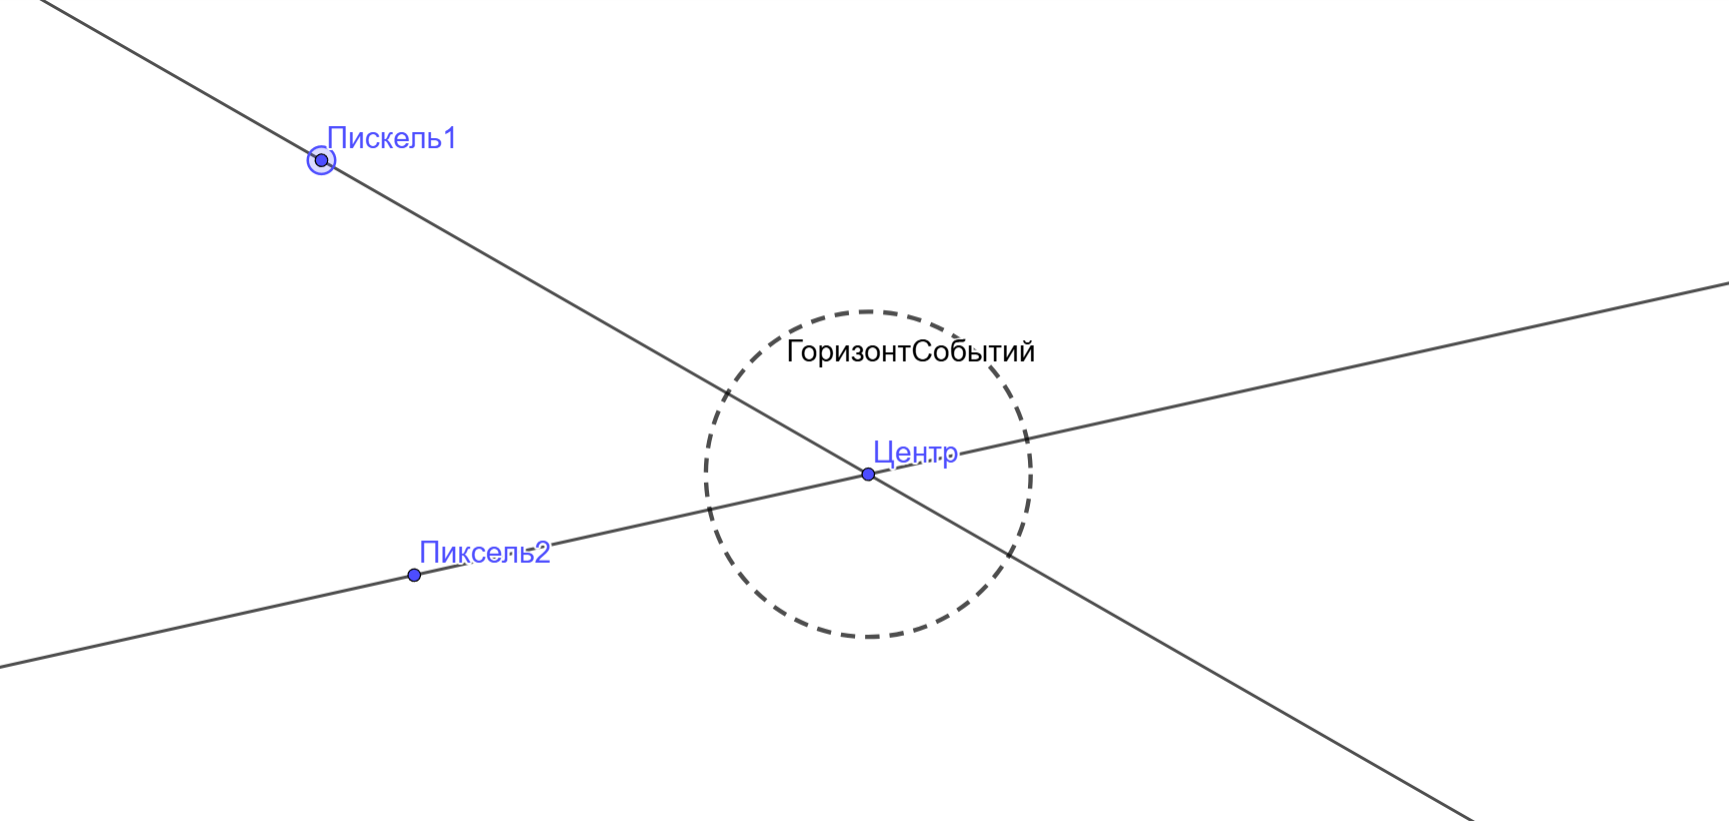
\includegraphics[width=1.0\linewidth]{rotation_plane}
    \caption{Разные плоскости вращения с точки зрения камеры.}
    \label{fig:rotation_plane}
\end{figure}

Без уменьшения общности примем $\phi_0 = 0$. Начальный радиус $r_0 = |\mathbf{a_c}|$, то есть начальный обратный радиус $u_0 = \frac{1}{r_0} = \frac{1}{|\mathbf{a_c}|}$. Таким образом первая компонента $\mathbf{y_0}$ определена.

Для нахождения второй компоненты сперва нужно определить вектор вращения луча $\mathbf{w_{nm}}$, то есть вектор, задающий плоскость вращения. В общем случае для каждого пикселя плоскость вращения будет отличаться (см. рис. \ref{fig:rotation_plane}).

\begin{equation}
\label{eq:w_ray}
    \mathbf{w_{nm}} = \mathbf{a_c} \times \mathbf{d_{nm}}.
\end{equation}

\newpage

\begin{figure}[h]
    \centering
    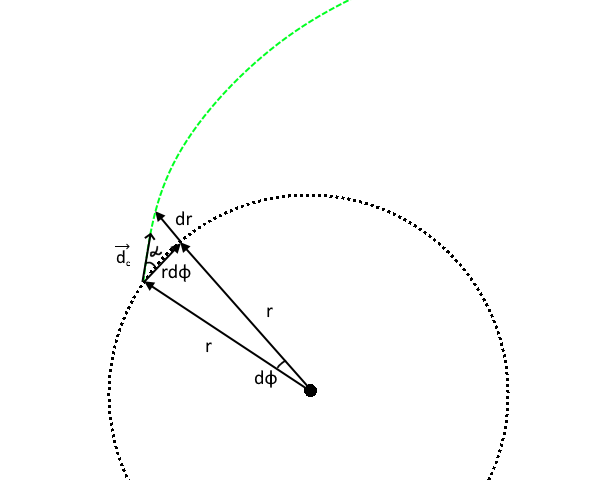
\includegraphics[width=0.8\linewidth]{BlackHole-RayAngle}
    \caption{Начальные условия (зеленым изображена траектория света, черным пунктиром - окружность, центр которой совпадает с центром черной дыры).}
    \label{fig:blackhole_rayAngle}
\end{figure}

Поскольку вторая компонента $\mathbf{y_0}$ это $\frac{du}{d\phi}$, то необходимо вычислить начальное значение этой производной. Пользуясь методом малых перемещений (см. рис. \ref{fig:blackhole_rayAngle}):

\begin{equation}
\label{eq:dudr_init}
    \left.\frac{du}{d\phi}\right|_{\phi=\phi_0=0} = \frac{d\left(\frac{1}{r}\right)}{d\phi} = -\frac{1}{r^2}\left(\frac{dr}{d\phi}\right) = -\frac{\tan{\alpha}}{r} = -\frac{1}{r}\left(\frac{\mathbf{a_c} \cdot \mathbf{d_{nm}}}{\left|\mathbf{w_{nm}}\right|}\right).
\end{equation}

Подытоживая, начальное условие $\mathbf{y_0}$ будет равно:

\begin{equation}
\label{eq:runge-kutte_y0}
    \mathbf{y_0} =
    \begin{cases}
        \frac{1}{\left|\mathbf{a_c}\right|}
        \\
        -\frac{1}{r}\left(\frac{\mathbf{a_c} \cdot \mathbf{d_{nm}}}{\left|\mathbf{w_{nm}}\right|}\right)
    \end{cases}
\end{equation}

\newpage

\subsection{Краевые случаи}
\label{subsec:corner_cases}
Для черной дыры выделяются два краевых случая:

\begin{enumerate}
    \item Попадание луча в горизонт событий.
    \item Уход луча на бесконечность.
\end{enumerate}

Рассмотрим каждые из них отдельно.

\subsubsection{Попадание луча в горизонт событий}
\label{subsubsec:events_horizon}

Луч, попавший в горизонт событий, уже никогда не выйдет из него, поэтому можно сказать, пользуясь законом обратимости света, что такие лучи приобретают черный цвет (если по пути до этого не пересеклись с другим объектом, разумеется).

Поскольку \textit{радиус Шварцшильда} $r_s$ является радиусом горизонта событий, то на каждой итерации решения уравнения \eqref{eq:diffur} методом Рунге-Кутты необходимо проводить проверку на нахождение внутри шара горизонта событий. То есть если на $i$-ой итерации, $r_i = \frac{1}{u_i} < r_s$, то нужно остановить итерирование и возвращать в качестве результата алгоритма рендеринга черной дыры полученный на предыдущих итерациях итоговый цвет.

\subsubsection{Уход луча на бесконечность}
\label{subsubsec:goes_to_infinity}

Луч, находящийся далеко от черной дыры, движется по почти прямой траектории. В таком случае можно считать, что направление луча не изменится, а значит можно сразу окрасить луч света в какой-то цвет на основании \textit{дальнего} окружения черной дыры.

\newpage

\begin{figure}[h]
    \centering
    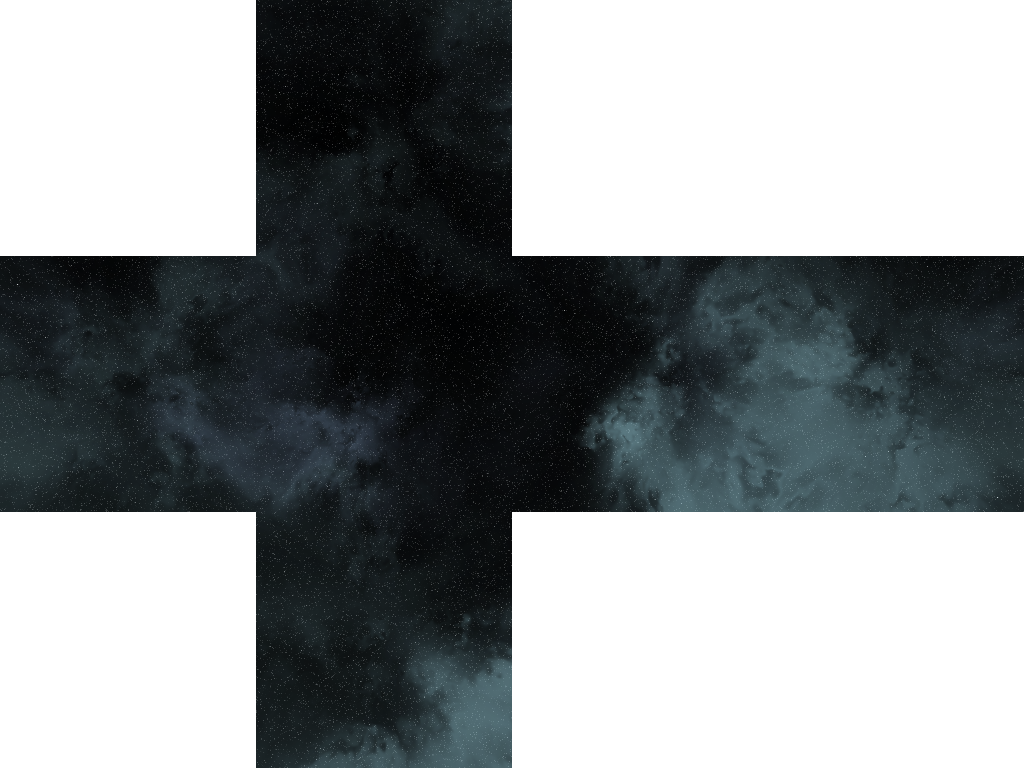
\includegraphics[width=1.0\linewidth]{cubemap}
    \caption{Кубическая текстура звездного неба.}
    \label{fig:cubemap}
\end{figure}

Черные дыры - это массивные объекты, находящиеся в космосе. Поэтому в качестве окружения разумно выбрать звездное небо (см. рис. \ref{fig:cubemap}) и в случае ухода луча на бесконечность брать значения, соответствующие направлению луча вдали от черной дыры. из этого звездного неба.

Осталось определить условие ухода луча на бесконечность. В общем случае на каждой $i$-ой итерации стоило бы проверять, как далеко свет ушел, но для черной дыры можно сделать упрощение, которое несет в себе еще и решение различных визуальных проблем: когда луч уходит все дальше и дальше от черной дыры, то $\phi$ из \eqref{eq:diffur} почти перестает меняться, что может вызывать проблемы с постоянным шагом $\Delta\phi$ в методе Рунге-Кутты. Упрощенное условие ухода на бесконечность выглядит следующим образом (см. рис. \ref{fig:blackhole_rayAngle}):

\begin{equation}
\label{eq:goes_to_infinity}
    \tan{\alpha} > tan_{crit} \quad \textit{или} \quad \left(\frac{du}{d\phi}\right)_i < -tan_{crit} \cdot u.
\end{equation}
, где $tan_{crit}$ - критическое значение тангенса угла $\alpha$ к окружности с центром, совпадающим с центром черной дыры.

\subsection{Аккреционный диск}
\label{subsec:accr_disk}

Все прошлые разделы описывали реализацию \textit{гравитационного линзирования}. Однако стоит отметить, что по соседству с черной дырой часто оказывается вращающийся горячий газовый диск, именуемый \textit{аккреционным диском}. Аккреционный диск по своим размерам сопоставим с радиусом Шварцшильда во всех направлениях (в том числе и в толщине) и поскольку это горячий газ, то его можно воспринимать как полупрозрачный объект.

Сложность визуализации аккреционного диска зависит от желаемого уровня реалистичности. Для данной работы достаточно ограничиться следующими параметрами аккреционного диска: вектор вращения диска $\mathbf{w_{accr}}$, внутренним $r_{min}$ и внешним $r_{max}$ радиусами, толщиной диска $H_{accr}$, а также цветом диска зависящим только от радиуса и расстоянием $h_{accr}$ от плоскости диска, задаваемой вектором вращения $\mathbf{w_{accr}}$. Этих параметров хватит для описания радиальной плотности $\rho_{accr}$ аккреционного диска:

\begin{equation}
\label{eq:accr_disk}
    \rho_{accr} = \max{\left(\text{noise}(r_{accr}) - \frac{\left|h_{accr}\right|)}{H_{accr}}, 0\right)},
    \quad
    r_{min} \le r_{accr} \le r_{max}.
\end{equation}
, где $r_{accr}$ - радиус в полярных координатах плоскости вращения аккреционного диска, а $\text{noise}(x)$ - функция плавной случайности, значения которой являются псевдослучайными, но при этом плавно меняются вдоль оси $x$.

Формулы для вычисления параметров $h_{accr}$ и $r_{accr}$ при известных декартовых координатах $\mathbf{a}$:

\begin{equation}
\label{eq:h_accr}
    h_{accr} = -\left(\mathbf{a} \cdot \mathbf{w_{accr}}\right)
\end{equation}

\begin{equation}
\label{eq:r_accr}
    r_{accr} = \left|\mathbf{a} + h_{accr}\mathbf{w_{accr}}\right|
\end{equation}

Плотность $\rho_{accr}$ используется на каждом шаге итерации, чтобы добавить плотность в данной точку итерации, помноженную на цвет аккреционного диска, к итоговому цвету.

\subsection{Переход из полярных координат плоскости вращения в декартовы}
\label{subsec:transition_from_polar_to_decart}

Для отрисовки аккреционного диска необходимо перейти из полярных координат $\left(\frac{1}{u}, \phi\right)$, в которых решается дифференциальное уравнение \eqref{eq:diffur} в декартовы $\left(\mathbf{a}, \mathbf{d}\right)$, где $\mathbf{a}$ - координаты луча, а $\mathbf{d}$ - направление луча. Это необходимо сделать, поскольку в декартовых координатах проще вычислить $r_{accr}$ и $h_{accr}$. Разумно разбить обсуждаемый переход на два последовательных этапа: поворот и масштабирование.

Поворот координат определяется начальным вектором, углом поворота и поскольку используются трехмерные декартовы координаты, то еще необходимо использовать вектор плоскости. Начальным вектором в данном случае будет нормализованный вектор позиции камеры $\mathbf{a_c}$ из раздела \ref{subsec:ray_init}, углом поворота будет угол $\phi$ из уравнения \eqref{eq:diffur}, а вектором плоскости - вектор вращения $\mathbf{w_{nm}}$ из все того же раздела \ref{subsec:ray_init}. Таким образом для искомой позиции $\mathbf{a}$ можно найти нормализованный вектор $\frac{\mathbf{a}}{\left|\mathbf{a}\right|}$ можно найти по следующей формуле:

\begin{equation}
\label{eq:rotate_pos}
    \frac{\mathbf{a}}{\left|\mathbf{a}\right|} = \left( \frac{\mathbf{a_{с}}}{\left|\mathbf{a_{с}}\right|} \right) \cdot \cos{\phi} + \left(\frac{\mathbf{w_{nm}}}{\left|\mathbf{w_{nm}}\right|} \times \frac{\mathbf{a_c}}{\left|\mathbf{a_c}\right|} \right) \cdot \sin{\phi}.
\end{equation}

Для нахождения вектора $\mathbf{a}$ нужно произвести масшитабирование, то есть домножить найденное в \eqref{eq:rotate_pos} на $\left|\mathbf{a}\right| = \frac{1}{u} = r$ - радиус.

\begin{figure}[h]
    \centering
    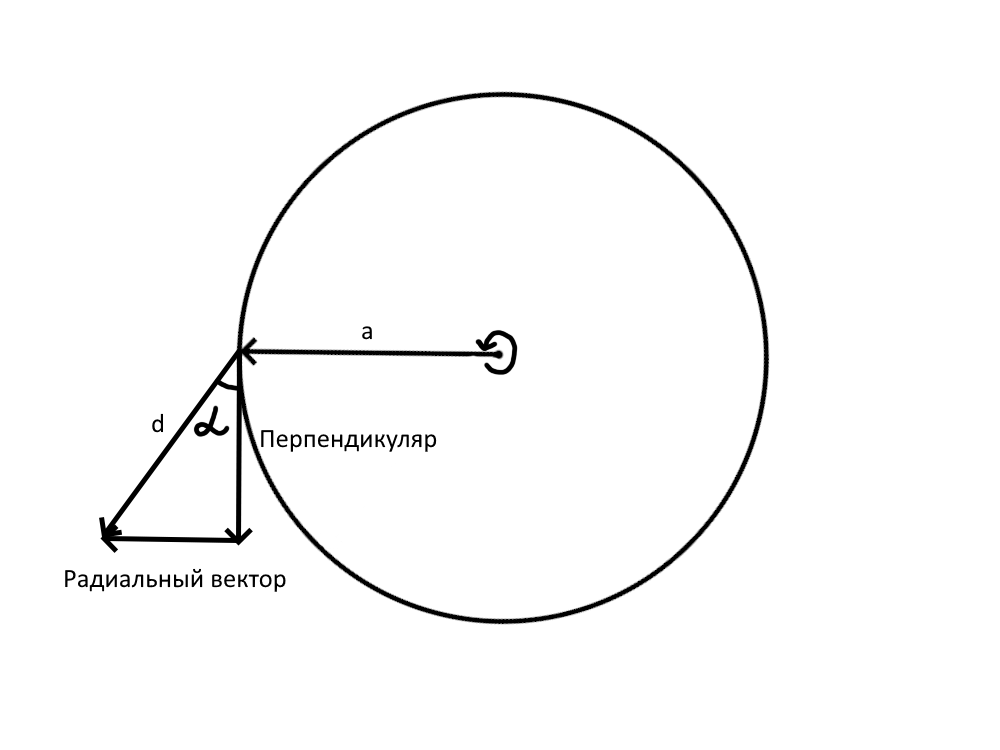
\includegraphics[width=0.7\linewidth]{TransformDirection}
    \caption{Перпендикуляр к движению луча (угловой вектор) и радиальный вектор направления $\mathbf{d}$.}
    \label{fig:transform_direction}
\end{figure}

Помимо найденной позиции $\mathbf{a}$ необходимо также найти направление $\mathbf{d}$ луча в точке $\mathbf{a}$:

\begin{equation}
\label{eq:rotate_dir}
    \mathbf{d} = \frac{\left(\frac{\mathbf{w_{nm}}}{\left|\mathbf{w_{nm}}\right|} \times \frac{\mathbf{a}}{\left|\mathbf{a}\right|}\right) - \mathbf{a}\left(\frac{du}{d\phi}\right)}{\left| \left(\frac{\mathbf{w_{nm}}}{\left|\mathbf{w_{nm}}\right|} \times \frac{\mathbf{a}}{\left|\mathbf{a}\right|}\right) - \mathbf{a}\left(\frac{du}{d\phi}\right) \right|}
\end{equation}
, где $\left(\frac{\mathbf{w_{nm}}}{\left|\mathbf{w_{nm}}\right|} \times \frac{\mathbf{a}}{\left|\mathbf{a}\right|}\right)$ - перпендикуляр к позиции $\mathbf{a}$ в плоскости вращения, направленный вдоль движения (угловой вектор направления $\mathbf{d}$), $\mathbf{a}\left(\frac{du}{d\phi}\right) = \frac{\mathbf{a}}{\left|\mathbf{a}\right|}\left(\frac{du}{d\phi} \cdot r\right) = \frac{\mathbf{a}}{\left|\mathbf{a}\right|} \tan{\alpha}$ - радиальный вектор направления $\mathbf{d}$ (см. рис. \ref{fig:transform_direction}). 

\subsection{Обзор итогового алгоритма}
\label{subsec:algos}

Итоговый алгоритм выглядит следующим образом:

\begin{enumerate}
\label{enum:algos}
    \item Инициализация лучей света (раздел \ref{subsec:ray_init}).
    \item Переход из декартовых координат в полярные координаты плоскости вращения (раздел \ref{subsec:transition_from_decart_to_polar}).
    \item В бесконечном цикле решения дифференциального уравнения методом Рунге-Кутты:
    \label{item:infinity_loop}
    \begin{enumerate}
        \item Проверка краевых случаев (раздел \ref{subsec:corner_cases}):
        \begin{enumerate}
            \item Проверка на нахождение в горизонте событий (раздел \ref{subsubsec:events_horizon}).
            \item Проверка на уход в бесконечность (раздел \ref{subsubsec:goes_to_infinity}).
            \label{item:goes_to_infinity}
        \end{enumerate}
        \item Получение новой точки итерации методом Рунге-Кутты (раздел \ref{subsec:runge-kutte}).
        \item Переход из полярных координат плоскости вращение в декартовы (раздел \ref{subsec:transition_from_polar_to_decart}).
        \item Добавление к итоговому цвету цвета аккреционного диска (раздел \ref{subsec:accr_disk}).
    \end{enumerate}
\end{enumerate}

Полученный алгоритм не следует реализовывать буквально в вышеописанном виде. Бесконечный цикл в пункте \ref{item:infinity_loop} необходимо сделать конечным, но с большой верхней границей количества итераций, поскольку лучи теоретически могут попасть в фотонную сферу - область вокруг черной дыры, в которой лучи двигаются по окружности бесконечно и таким образом не достигая краевых случаев. По этой причине окончание конечного цикла стоит обработать отдельно. В данной работе обработка такая же, как и в случае с уходом в бесконечность в пункте \ref{item:goes_to_infinity}.

Итоговый алгоритм является примером \textit{марширования лучей} \linebreak\textit{(ray marching)}.

\begin{figure}[h]
    \centering
    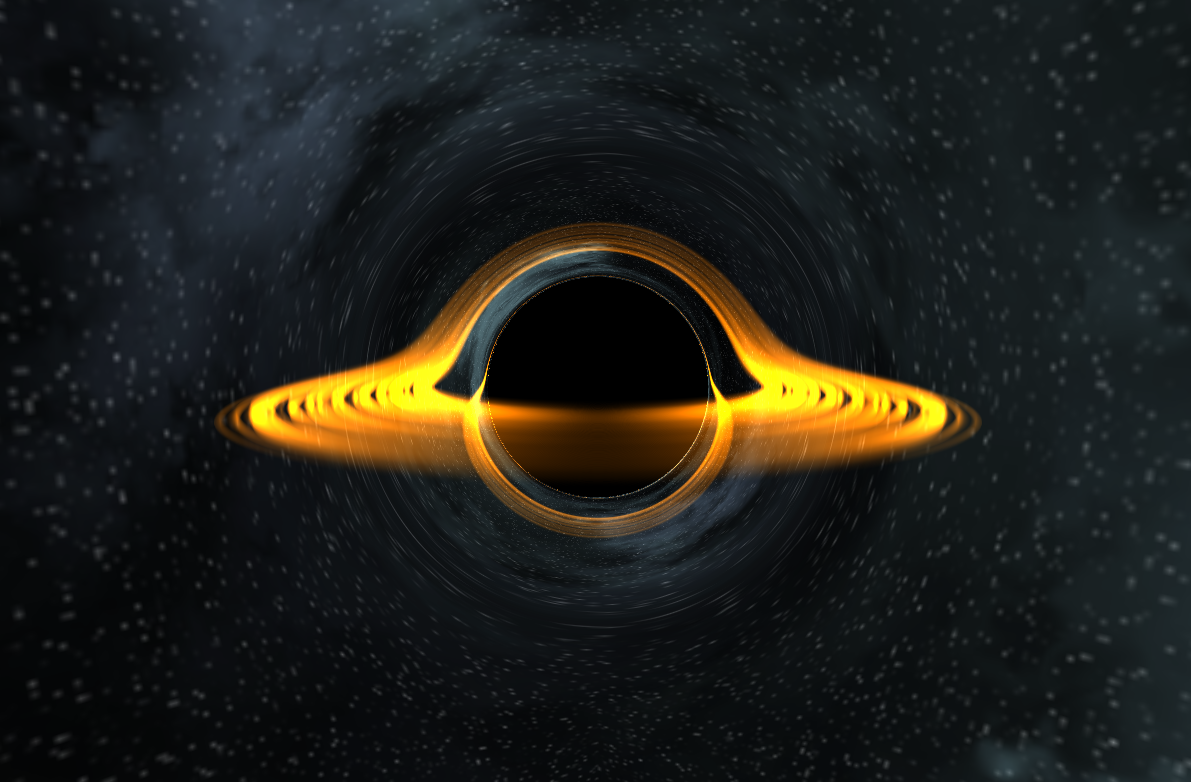
\includegraphics[width=1.0\linewidth]{BlackHoleRayMarching}
    \caption{Рендеринг черной дыры с использованием марширования лучей.}
    \label{fig:black_hole_ray_marching}
\end{figure}

\newpage
